In this chapter, we propose two new tasks to evaluate our knowledge-aware NLU pipeline. The first task is semantic anomaly detection in newswire headlines.

\section{Understanding Events}
Understanding events is a fundamental prerequisite for deeper semantic 
analysis of language.  We introduce the problem of automatic anomalous event
detection
in this chapter and propose a novel event model that can learn to differentiate
between normal
and anomalous events.  We generally define anomalous events as those that are
unusual compared
to the general state of affairs and might invoke surprise when reported.  For
example, given the 
following event mention 
\begin{itemize}
 \item[] \textit{Many of them blessed themselves by an endless cycle of bombings
and  shootings and massacres.}
\end{itemize}
one might think it is strange because \textit{them} refers to people, people
usually do not \textit{bless themselves} by \textit{bombings and
shootings 
and massacres}, let alone an \textit{endless cycle} of them.  But the mentions
\begin{itemize}
 \item[] \textit{Many of them blessed themselves by regular visits to the
church.}
 \item[] \textit{Many of them caused large scale destruction by an endless cycle
of bombings and shootings and massacres.}
\end{itemize}
are not as unusual as the previous one.  While all three sentences are equally
valid syntactically, it 
is our knowledge about the role fillers 
---both individually and specifically in combination---  
that enables us to 
differentiate between normal and anomalous events.  Hence we hypothesize that
\emph{anomaly is a result of unexpected or 
unusual combination of semantic role fillers}.

Given this idea, an automatic
anomaly detection algorithm has to encode
the goodness of semantic role filler coherence.  This is a hard problem since
determining what a good combination of role fillers is 
requires deep semantic and pragmatic knowledge.  
Moreover, manual judgment of anomaly itself may be difficult and people often
may not agree with each other in this
regard.  We describe the difficulty in human judgment in greater detail in
Section~\ref{sec:annot}.  
Automatic detection of anomaly requires encoding complex information, which
poses the challenge of sparsity
due to the discrete representations of meaning, that are words.  These problems
range from polysemy and synonymy at the 
lexical semantic level to entity and event coreference at the discourse level.

\subsection{Data}
We crawl 3684 ``weird news'' headlines available publicly 
on the website of NBC
news\footnote{\url{
http://www.nbcnews.com/html/msnbc/3027113/3032524/4429950/4429950_1.html}}, 
such as the following: 
\begin{itemize}
 \item \textit{India weaponizes world's hottest chili.}
 \item \textit{Man recovering after being shot by his dog.}
 \item \textit{Thai snake charmer puckers up to 19 cobras.}
\end{itemize}
We assume that the events extracted from this source, called NBC Weird Events
(NWE) henceforth, are
anomalous for training.  NWE contains 4271 events extracted using 
SENNA's SRL.  We use 3771 of those events as our negative training data. 
Similarly, we extract events also from
headlines in the AFE section of Gigaword, called Gigaword Events (GWE)
henceforth.  We assume these events are normal.
To use as positive examples for training event composition, we sample roughly
the same number of events from 
GWE as our negative examples from NWE. From the two sets, we uniformly sample 1003 events
as the test set and validate the labels by getting crowd-sourced annotations.

\subsection{Annotation}
We post the annotation of the test set containing 1003 events as
Human Intelligence Tasks (HIT) on Amazon Mechanical Turk (AMT).
We break the task into 20 HITs and ask the workers to select one of the 
four options - \textit{highly unusual}, \textit{strange}, \textit{normal} and 
\textit{cannot say} for each event.  We ask them to select \textit{highly
unusual} when the 
event seems too strange to be true, \textit{strange} if it seems unusual but 
still plausible, and \textit{cannot say} only if the information present in the 
event is not sufficient to make a decision.  We publicly release this set of 1003
annotated events for evaluating future research.

\begin{table}
\begin{center}
  \begin{tabular}[c]{|c|c|}
 \hline
  Total number of annotators & 22\\
  \hline
  \textit{Normal} annotations & 56.3\% \\
  \hline
  \textit{Strange} annotations & 28.6\% \\
  \hline
  \textit{Highly unusual} annotations & 10.3\% \\
  \hline
  \textit{Cannot Say} annotations & 4.8\% \\
  \hline
  Avg. events annotated per worker & 344 \\
  \hline
  4-way Inter annotator agreement ($\alpha$) & 0.34 \\
  \hline
  3-way Inter annotator agreement ($\alpha$) & 0.56 \\
  \hline
  \end{tabular}
\end{center}
 \caption{Annotation Statistics}
 \label{table:annot}
\end{table}
Table~\ref{table:annot} shows some statistics of the annotation task.  We
compute the Inter Annotator
Agreement (IAA) in terms of Kripendorff's alpha \cite{krippendorff1980content}. 
The advantage of using this
measure instead of the more popular Kappa is that the former can deal with
missing information, which is the case with
our task since annotators work on different overlapping subsets of the test set.
 The 4-way IAA shown in the table 
corresponds to agreement over the original 4-way decision (including
\textit{cannot say}' while the 3-way IAA is measured after merging the 
\textit{highly unusual} and \textit{strange} decisions.  

Additionally we use
MACE \cite{hovy2013learning} to assess the quality of 
annotation.  MACE models the annotation task as a generative process of
producing the observed labels conditioned on the 
true labels and the competence of the annotators, and predicts both the latent
variables.  The average of competence of annotators, 
a value that ranges from 0 to 1, for our task is 0.49 for the 4-way decision and
0.59 for the 3-way decision.  

We generate
true label predictions produced by MACE, discard the events for which the
prediction remains to be \textit{cannot say}, and use the 
rest as the final labeled test set.  This leaves 949 events as our test dataset,
of which only 41\% of the labels are \textit{strange} or \textit{highly
unusual}.  It has to be noted that even though our test set 
has equal size samples from both NWE and GWE, the true distribution is not
uniform.

\subsection{Model for Semantic Anomaly Detection}
We now describe our Neural Event Model (NEM) for encoding events. Events encoded using this model are then passed to a multi-layer perceptron
for making the anomaly decision. We define an event as the pair $(V, \textbf{A})$, where $V$
is a semantic verb\footnote{By semantic verb, we mean an action word whose
syntactic category is not necessarily a verb.  
For example, in \textit{Terrorist attacks on the World Trade Center..},
\textit{attacks} is not a verb but is still an 
action word.}, and $\textbf{A}$ is the set of its semantic arguments like agent,
patient, time, location, so on. Our aim
is to obtain a vector representation of the event that is composed from
representations of individual words, while explicitly guided by the semantic
role structure.
This representation can be understood as an embedding of the
event
in an event space.  

\subsubsection{Encoder}
Neural Event Model (NEM) is a kind of RNN
that is guided by a tree representation of events like the one shown in
Figure~\ref{fig:nem_event_tree}.  The edges 
connected to the root of the tree correspond to the verb and its semantic roles
(arguments).  All the other edges form binary sub-trees of arguments.  
\begin{figure}
  \begin{center}
  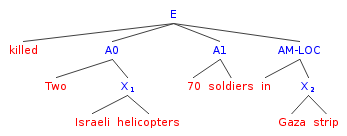
\includegraphics[width=4in]{figures/event_tree.png}
  \caption{Example of an event tree}
  \label{fig:nem_event_tree}
  \end{center}
 \end{figure}
NEM is a supervised model that learns to differentiate between anomalous and
normal events by 
classifying the event embeddings.  
The inputs to NEM are the semantic arguments, and the representations of words
in 
each argument.  We recursively compose the words in each argument to obtain
argument level
representations, which are then composed to obtain an event embedding. 

Intra-argument composition 
(called argument composition henceforth) is unsupervised, and we use contrastive
estimation 
to learn the parameters.  The structure of the binary tree backing
argument composition is determined dynamically, composing at each stage the two
nodes
which give the best composition score.  Inter-argument 
composition (called event composition henceforth) is supervised
and we use label error to learn the parameters.  Figure~\ref{fig:nem}
shows how NEM encodes the event shown in Figure~\ref{fig:nem_event_tree}.  The blue
boxes show argument composition 
and the red box shows event composition.  
\begin{figure}
  \begin{center}
  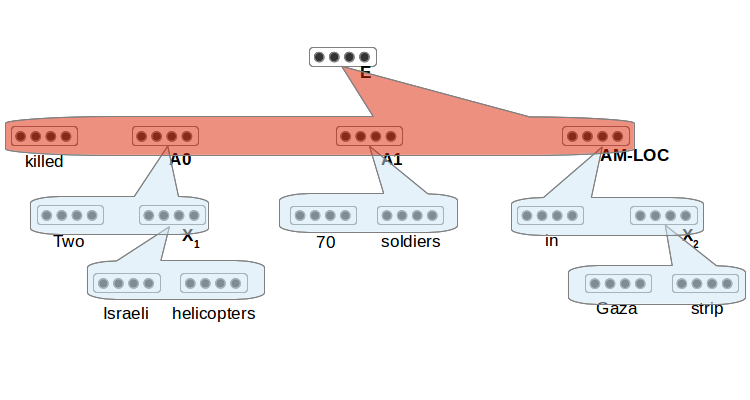
\includegraphics[width=4in]{figures/nem2.png}
  \caption{Neural Event Model: Encoding}
  \label{fig:nem}
  \end{center}
\end{figure}
\subsection{Training}
NEM is trained in two phases.  The first, argument composition is unsupervised 
while the second, event composition is supervised.
\paragraph{Argument Composition}
An argument composition node takes inputs of dimensionality $2n$ and produces an
composed output representation
of dimensionality $n$ and a composition score.  Accordingly, we define the node
in terms of the parameters $\theta_{arg} = \{W_{arg} \in \mathbb{R}^{n \times 2n}; b_{arg}, S_{arg} \in
\mathbb{R}^{n \times 1}; V\}$
where $W_{arg}$, $b_{arg}$ and $S_{arg}$ are the composition weight, bias and
the scoring operators respectively 
as described previously, and $V$ is the set of representations of all the words
in the vocabulary.  
All nodes performing argument composition use the same parameters.  Training is
done in contrastive estimation fashion
and the objective is 
\begin{equation*}
 \argmin_{\theta_{arg}} J_{arg} = \argmin_{\theta_{arg}} max(0, 1-s+s_c)
\end{equation*}
where $s$ is the score of the composition of the entire argument produced by 
the root node of the argument, and $s_c$ is the score produced by randomly
replacing one of the words in the argument at a time. 
\paragraph{Event Composition}
Event composition takes argument representations and produces the event
representation and label indicating whether the event is
normal or anomalous.  We define the event composition node in terms of the
parameters $\theta_{event} = \{W_{event} \in \mathbb{R}^{n \times kn}; b_{event},
L_{event} \in \mathbb{R}^{n \times 1}\}$
where $k$ is the number of semantic arguments per event.  $L_{event}$ is the
label operator.  The objective of this
phase is 
\begin{align*}
\begin{aligned}
\argmin_{\theta_{event}} J_{event} = \argmin_{\theta_{event}} \left( - l \log h(e) + (1-l) \log (1 - h(e)) \right)
\end{aligned}
\end{align*}
where $l$ is the reference binary label indicating whether the event is normal or
anomalous, $e$ is the event representation and
$h(e)$ is the output of the logistic function.  Concretely,
\begin{equation*}
 h(e) = \frac{1}{1+e^{-L_{event}^\intercal e}}
\end{equation*}
We implement the functions and perform stochastic gradient descent using Theano
\cite{bergstra2010theano}.

\subsection{Results}
We evaluate the performance of event composition by comparing the predicted
labels from the classifier against the ones given by MACE.
We merge the two anomaly classes and calculate accuracy of the binary
classifier, and the precision and recall of anomaly detection.
\begin{table}
\begin{center}
  \begin{tabular}[c]{|c|c|c|}
 \hline
 \multicolumn{2}{|c|}{Accuracy} & 65.44\% \\
 \hline
 \multirow{2}{*}{Anomalous} & Precision & 56.55\% \\
 \cline{2-3}
 & Recall & 48.22\% \\
 \hline
 \multirow{2}{*}{Normal} & Precision & 64.62\% \\
 \cline{2-3}
 & Recall & 77.66\% \\
 \hline
  \end{tabular}
\end{center}
 \caption{Classification Performance}
 \label{table:res1}
\end{table}
Table~\ref{table:res1} shows these results.  It can be noted that the accuracy
is significantly higher than a random 
expectation of 50\%.  The precision of a random classifier in predicting
anomalous events is expected to be 41\%, since 
that is the percentage of anomaly labels in our reference set as described in
Section~\ref{sec:annot}.

\subsection{Proposed Work}

\section{Understanding Experiments}
\subsection{Data}
\subsection{Proposed Work}